\documentclass[11pt]{article}
\usepackage[margin=0.78in]{geometry}
\usepackage{graphicx}
\usepackage{amsmath,amssymb}
\usepackage{booktabs}
\usepackage{url}
\usepackage[numbers,sort&compress]{natbib}
\usepackage{authblk}
\usepackage{hyperref}
\hypersetup{colorlinks=true,linkcolor=black,citecolor=black,urlcolor=blue}
\setlength{\parskip}{0.55em}
\setlength{\parindent}{0pt}

\title{Teacher-guided corrective residuals support reflex-like recovery in simulated locomotion}
\author[1,*]{Andr\'es de Vicente}
\author[1,*]{Renee Vieira}
\author[1,*]{Charlie Hou}
\affil[1]{Neuromatch Impact Scholars Program, Team RNNematode}
\affil[*]{Equal contribution}
\date{2026}

\begin{document}
\maketitle

\textbf{Keywords:} motor control; cerebellum; residual policy; reinforcement learning; locomotion; reflexes; BrainCAD

\begin{abstract}
Animals do not recover from every stumble by relearning a motor policy.  Recovery is more naturally described as layered control: an ongoing motor command is combined with faster corrective pathways shaped by error and practice.  We tested this idea in BrainCAD, a biologically inspired neural-control toolkit built around MuJoCo locomotion experiments.  Several reinforcement-learning-only corrective circuits, including spinal gain gating and residual modules, did not learn reliable fast recovery under PPO.  A cerebellar-inspired residual became effective only when trained with a direct teacher signal.  This is close to residual policy learning and policy distillation \citep{johannink2018residualrl,rusu2015policydistillation,schmitt2018kickstarting}; the contribution is not a new distillation algorithm, but a controlled demonstration that this learning signal was necessary in our biologically inspired locomotor-control architecture.  In Humanoid-v4, the same trained checkpoint was evaluated with the residual switched on and off under identical perturbation schedules.  Across 20 seeds, the residual reduced fall AUC by 0.361 on average and increased return AUC by 74.6.  The correction could also be distilled into a cortex-only policy, preserving most of the fall reduction.  Cross-body experiments showed strong effects in Humanoid, Walker2d, and Ant, with Hopper as a boundary case where stability gains were less clean and return often decreased.  These results suggest that biologically inspired corrective modules require an appropriately structured learning signal, not just an anatomically motivated architecture.
\end{abstract}

\section*{Introduction}
Reflexes are often described as simple loops, but real movement is not simple.  A body with many joints and contacts has many ways to fail: a foot can slip, sensory input can become unreliable, or a shove can arrive while the controller is already committed to a step.  Nervous systems solve this with layered circuits.  Spinal circuits provide fast sensorimotor pathways, cortex supports flexible voluntary control, and the cerebellum is strongly associated with internal models and error-based motor adaptation \citep{wolpert1998internalmodels,ito2008control,seidler2013errorbased}.

Motivated by this organization, we implemented several corrective circuits in BrainCAD \citep{braincad2026software} and tested them in ReflexBench, a perturbation suite for MuJoCo locomotion.  The first lesson was negative: PPO alone \citep{schulman2017ppo} often failed to discover a small, fast corrective action, even when the architecture was biologically plausible.  The successful variant used a teacher.  A robust policy was first trained under perturbations, and a cerebellar residual was then trained to imitate the teacher's correction relative to a nominal cortex, following the broad logic of residual policy learning and distillation \citep{johannink2018residualrl,rusu2015policydistillation,schmitt2018kickstarting}.  We therefore frame the result as a learning-signal result, not as evidence for a new principle of cerebellar biology.

\section*{Model}
The model has three pieces.  A cortex policy proposes a base action,
\[
u_t^{ctx} = \pi_\theta(o_t),
\]
where $o_t$ is the observation.  A teacher policy, trained separately with perturbations, produces $u_t^{teacher}$.  During imitation, the cerebellar residual is trained toward
\[
\Delta u_t^* = u_t^{teacher} - u_t^{ctx}.
\]
At evaluation time, the residual controller executes
\[
u_t = \mathrm{clip}\left(u_t^{ctx} + \alpha_t \Delta u_t, u_{min}, u_{max}\right),
\]
where $\alpha_t \in [0,1]$ is an optional engagement gate.  A later consolidation step removes the residual machinery by training a new cortex to imitate the final action $u_t$ directly.

\begin{figure}[t]
\centering
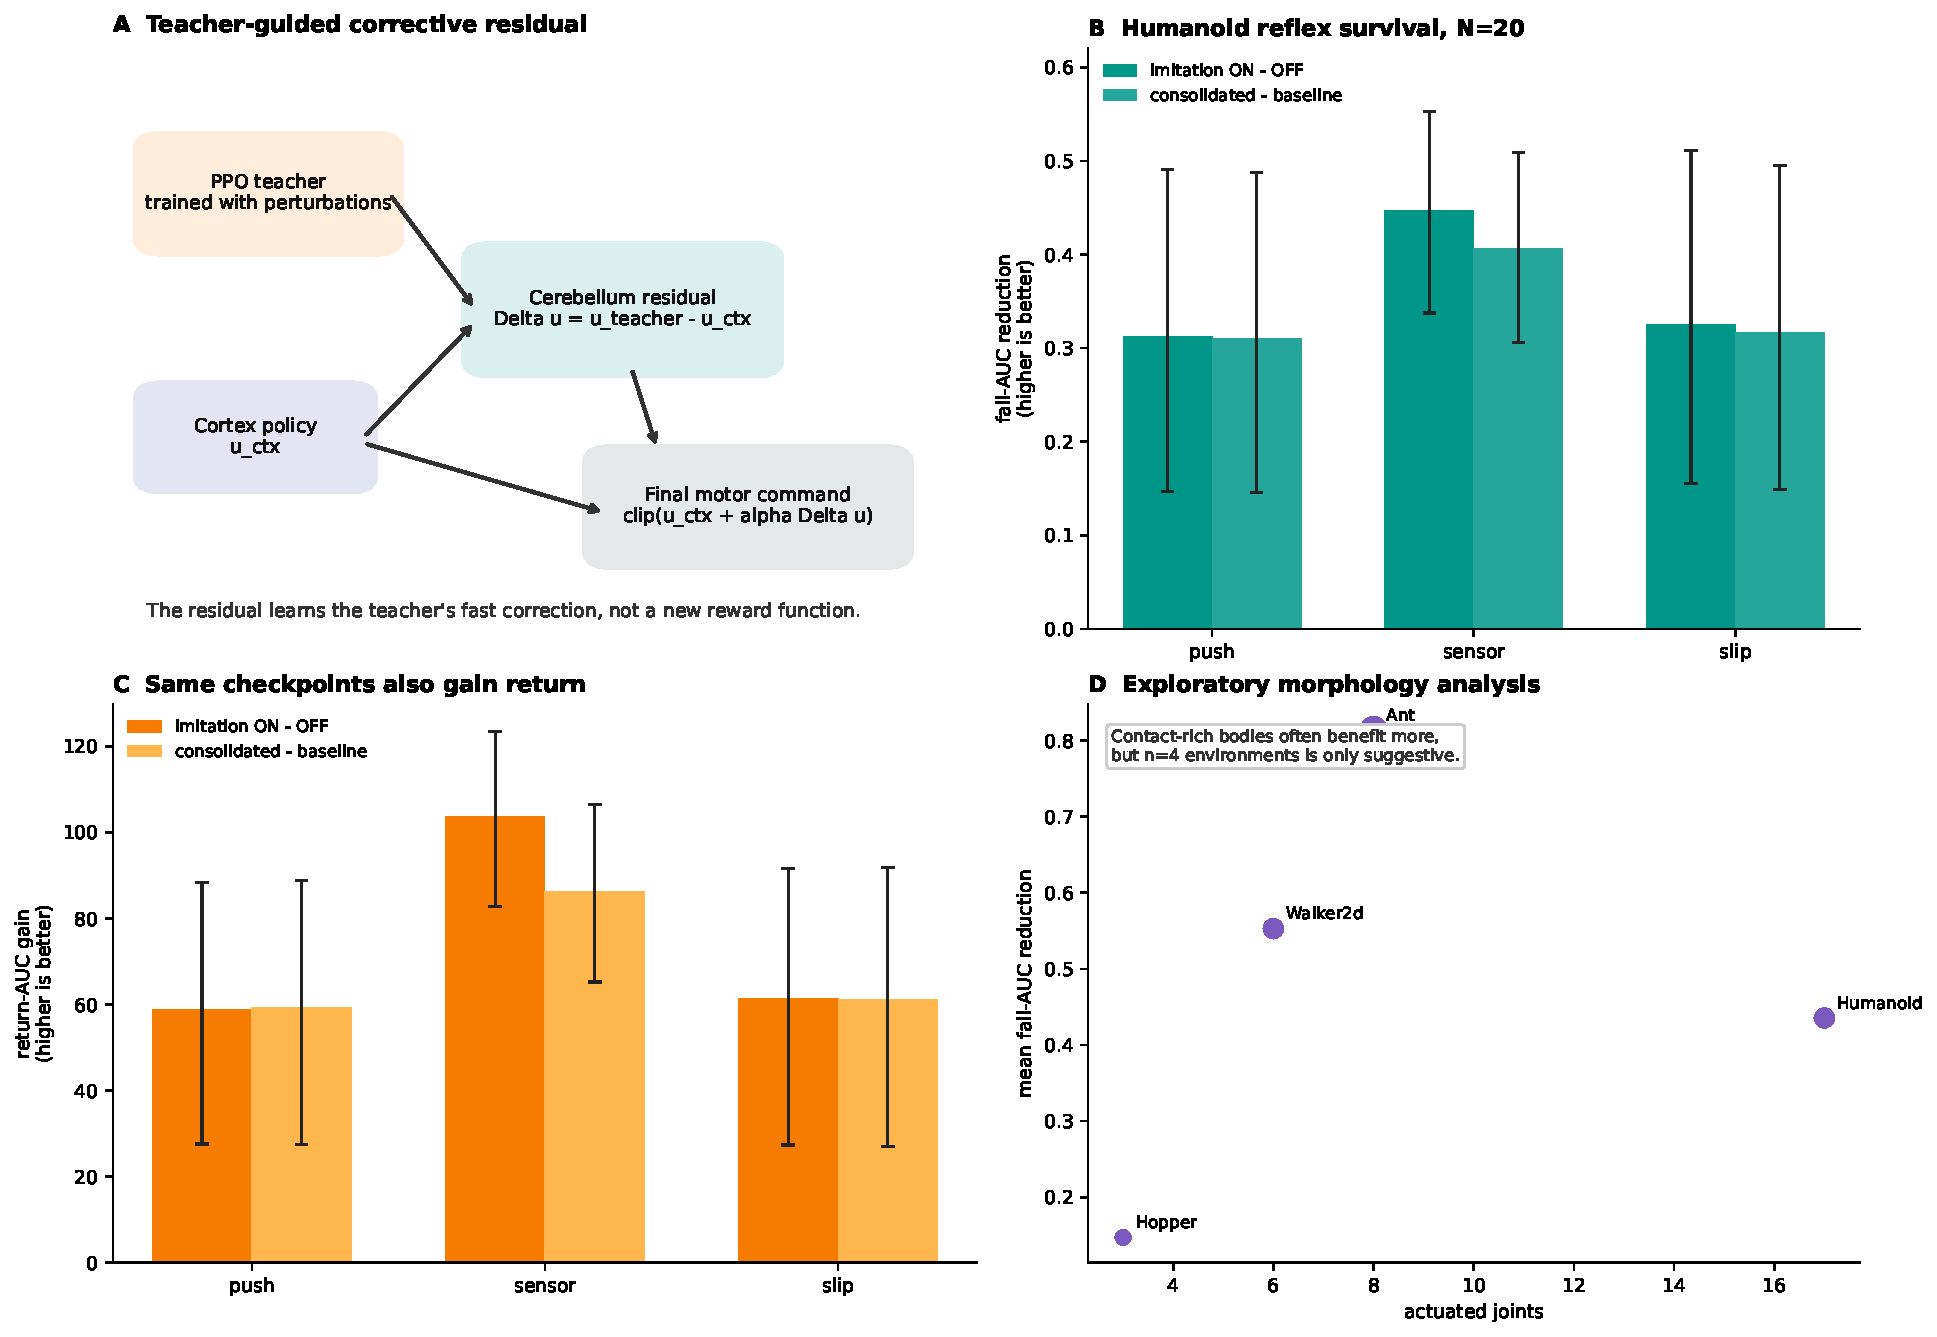
\includegraphics[width=\linewidth]{Figures/RNNematode-Figures.pdf}
\caption{\textbf{Teacher-guided residual control and main results.}  A, a perturbation-trained teacher supplies a corrective target for a cerebellar residual.  B, in Humanoid-v4, residual ON vs OFF evaluation with the same checkpoint reduces fall AUC across pushes, sensor corruption, and slips (N=20).  C, the same comparison improves return AUC.  D, cross-body results are suggestive of a morphology effect: contact-rich bodies benefit strongly, while Hopper remains a boundary condition. Points are mean estimates without confidence regions and are shown only as an exploratory morphology summary.}
\end{figure}

\section*{Results}
\textbf{RL-only correction was not enough.}  We first tested spinal gain gating, residual correction trained only by PPO, curriculum perturbations, basal-ganglia-like engagement gates, and stability auxiliary terms.  These variants were useful diagnostics, but none gave a reliable causal reduction in fall AUC.  Thus, the circuit diagram alone was not the main explanation.  The key variable was whether the module received enough information to learn a useful correction at the right time.

\textbf{Teacher-guided residuals improved survival.}  The teacher-guided residual was tested causally: the same checkpoint and the same perturbation schedule were evaluated with the residual enabled or disabled.  In the N=20 Humanoid campaign, fall AUC decreased for push (-0.313, 95\% CI [-0.491, -0.147]), sensor (-0.447, 95\% CI [-0.553, -0.338]), and slip (-0.325, 95\% CI [-0.511, -0.155]) perturbations, where negative numbers mean fewer falls.  Return AUC increased for push (58.8, 95\% CI [27.6, 88.4]), sensor (103.6, 95\% CI [82.7, 123.5]), and slip (61.4, 95\% CI [27.4, 91.6]).  Perturbation sanity checks verified that pushes, friction changes, and sensor corruption were actually applied, not only logged.

\textbf{Teacher quality mattered.}  A strong teacher produced stabilizing residuals.  A deliberately weak teacher produced residuals that could become harmful.  This argues against a simple capacity explanation: the student learned a direction of correction from the teacher, and a bad teacher could teach the wrong direction.

\textbf{Corrections could be consolidated.}  We trained a cortex-only policy to imitate the final action of the residual controller.  This consolidated policy no longer used an online cerebellar residual, but it retained most of the fall reduction in Humanoid and generalized under a long-push schedule.  This suggests that the residual pathway can act as a training scaffold: useful during learning, but not always necessary at inference.

\section*{Exploratory morphology analysis}
The cross-body pattern gives a useful intuition, but it should not be read as an evolutionary result.  Bodies with more actuators and richer contacts create more ways to nearly fall.  In those bodies, a separate corrective pathway may be valuable because the nominal policy cannot cover every recovery case cleanly.  Ant and Humanoid showed strong fall reductions, Walker2d also replicated, and Hopper exposed a stability--performance tradeoff.  This supports a modest morphology-dependent control hypothesis: layered corrections may become more useful as the body creates more recovery states for the controller to handle.

\section*{Methods in brief}
Experiments used BrainCAD with MuJoCo locomotion environments \citep{todorov2012mujoco,brockman2016openai}.  ReflexBench applied external pushes, friction reductions, and observation corruption.  Fall AUC was computed as the area under the fall-probability curve across the predefined perturbation-severity grid (Humanoid: push magnitudes 0--1 crossed with duration, slip severities 0--1.25 crossed with patch settings, and sensor dropout bursts 0--0.4).  Return AUC was computed analogously from mean return across the same severity grid.  Curves were computed per seed before paired ON--OFF deltas were summarized with bootstrap confidence intervals.  Lower fall AUC and recovery AUC are better, while higher return AUC is better.  Source notebooks and validation summaries are included in the micropublication package.

\section*{Data and code availability}
Code, notebooks, figures, validation files, and video indices are packaged with this submission.  The public repository is available at https://github.com/andrestrocyte/rnnematode-micropublication.  The original implementation uses the BrainCAD experiment structure, including circuit templates, MuJoCo wrappers, evaluation scripts, and video export.

\section*{Acknowledgments}
We thank Raymond Chua for senior mentorship, scientific guidance, and feedback on motor-control framing.  We also acknowledge the BrainCAD/NCAP software infrastructure used for circuit templates, MuJoCo wrappers, evaluation, and video export.

\bibliographystyle{plainnat}
\bibliography{references}
\end{document}
